Communication,
audiovisuel,
transports,
médecine:
tous ces domaines se sont transformés dans les dernières décennies,
en particulier grâce à la révolution numérique.
En effet le plus petit appareil électrique contient maintenant des composants
matériels programmables.

En 2013, on pense bien sûr aux téléphones portables dont la fonctionnalité et la
complexité les rapprochent des ordinateurs de bureau. Par exemple, le système
d'exploitation Android de Google est fondé sur le noyau Linux, destiné à la base
aux micro-ordinateurs.

Le noyau d'un système d'exploitation est chargé de faire l'intermédiaire entre
le matériel (processeur, mémoire, périphériques, …) et les applications
exécutées sur celui-ci (par exemple un navigateur web, une calculatrice ou un
carnet d'adresses).

Il doit aussi garantir la sécurité de celles-ci: en tant qu'intermédiaire de
confiance, le noyau a un certain nombre de responsabilités et est le seul à
avoir accès à certaines informations sensibles. Il est capital de s'assurer
qu'il est bien le seul à pouvoir y accéder. En particulier, il faut pouvoir
vérifier que les requêtes faites par l'utilisateur au noyau ne peuvent pas
volontairement ou involontairement détourner ce dernier et lui faire fuiter des
informations confidentielles.

Le problème est que, comme tous les logiciels, les noyaux de système
d'exploitation sont écrits par des humains qui ne sont pas parfaits. Les
activités de relecture et de débogage ont beau prendre la majeure partie du
temps de développement, il est facile de laisser passer des défauts de
programmation.

Ces erreurs, ou \emph{bugs}, peuvent avoir des conséquences dramatiques sur le
plan matériel ou humain. À titre d'exemple, un Airbus A320 embarque près de 10
millions de lignes de code: il est capital de vérifier que celles-ci ne peuvent
pas mettre en danger la sûreté des passagers.

Une technique efficace est de réaliser des tests, c'est-à-dire exécuter le
programme sous un environnement contrôlé. On peut alors détecter des
comportements non désirés. Mais même avec une grande quantité de tests il n'est
pas possible de couvrir tous les cas d'utilisation.

Une autre approche est d'analyser le code source du programme avant de
l'exécuter et de refuser de lancer les programmes qui contiennent certaines
constructions dangereuses. C'est l'analyse statique de programmes.

Une des techniques d'analyse statique les plus répandues et les plus simples est
le typage statique, qui consiste à associer, à chaque morceau de programme, une
étiquette décrivant quel genre de valeur sera produite par son évaluation. Par
exemple, si $n$ est le nom d'une variable entière, alors $n + 2$ produira
toujours une valeur entière.
Cela permet de savoir si les programmes manipuleront des données incompatibles
entre elles.

Pour en revenir aux noyaux de système d'exploitation, ceux-ci manipulent à la
fois des données sensibles et des données provenant du monde extérieur, pour
lesquelles on n'a aucune garantie. On veut pouvoir distinguer celles-ci.

Plus précisément, un des points cruciaux pour garantir l'isolation d'un noyau de
système d'exploitation est de restreindre la manière dont sont traitées les
informations provenant des programmes utilisateur.

Le but de cette thèse est de montrer que le typage statique peut être utilisé
pour détecter et interdire ces manipulations dangereuses.

\section{Rôle d'un système d'exploitation}

Un ordinateur est constitué de nombreux composants matériels: microprocesseur,
mémoire, et divers périphériques. Et au niveau de l'utilisateur, des dizaines de
logiciels permettent d'effectuer toutes sortes de calculs et de communications.
Le système d'exploitation permet de faire l'interface entre ces aspects.

Au cours de l'histoire des systèmes informatiques, la manière de les programmer
a beaucoup évolué. Au départ, les programmeurs avaient accès au matériel dans
son intégralité: toute la mémoire pouvait être accédée, toutes les instructions
pouvaient être utilisées.

Néanmoins c'est un peu restrictif, puisque cela ne permet qu'à une personne
d'interagir avec le système. Dans la seconde moitié des années 1960, sont
apparus les premiers systèmes «à temps partagé», permettant à plusieurs
utilisateurs de travailler en même temps.

Permettre l'exécution de plusieurs programmes en même temps est une idée
révolutionnaire, mais elle n'est pas sans difficultés techniques: en effet les
ressources de la machine doivent être aussi partagées entre les utilisateurs et
les programmes. Par exemple, plusieurs programmes vont utiliser le processeur
les uns à la suite des autres; et chaque programme aura à sa disposition une
partie de la mémoire principale, ou du disque dur.

Si plusieurs programmes s'exécutent de manière concurrente sur le même matériel,
il faut s'assurer que l'un ne puisse pas écrire dans la mémoire de l'autre, et
aussi que les deux n'utilisent pas la carte réseau en même temps. Ce sont des
rôles du système d'exploitation.

Ainsi, au lieu d'accéder directement au matériel via des instructions de bas
niveau, les programmes communiquent avec le noyau, qui centralise donc les
appels au matériel, et abstrait certaines opérations.

Par exemple, comparons ce qui se passe concrètement lors de la copie de données
depuis un cédérom ou une clef USB.\@

\begin{itemize}

  \item Dans le cas du cédérom, il faut interroger le bus SATA, interroger le
    lecteur sur la présence d'un disque dans le lecteur, activer le moteur,
    calculer le numéro de trame des données sur le disque, demander la lecture,
    puis déclencher une copie de la mémoire.

  \item Avec une clef, il faut interroger le bus USB, rechercher le bon numéro
    de périphérique, le bon numéro de canal dans celui-ci, lui appliquer une
    commande de lecture au bon numéro de bloc, puis copier la mémoire.

\end{itemize}

Ces deux opérations, bien qu'elles aient la même intention (copier de la mémoire
depuis un périphérique amovible), ne sont pas effectuées en extension de la même
manière. C'est pourquoi le système d'exploitation fournit les notions de
fichier, lecteur, etc: le programmeur n'a plus qu'à utiliser des commandes de
haut niveau («monter un lecteur», «ouvrir un fichier», «lire dans un
fichier») et, selon le type de lecteur, le système d'exploitation effectuera les
actions appropriées.

En résumé, un système d'exploitation est l'intermédiaire entre le logiciel et le
matériel, et en particulier est responsable de la gestion de la mémoire, des
périphériques et des processus. Les détails d'implantation ne sont pas présentés
à l'utilisateur; à la place, il manipule des abstractions, comme la notion de
fichier. Pour une explication détaillée du concept de système d'exploitation
ainsi que des cas d'étude, on pourra se référer à~\cite{tanenbaum}.

\section{Séparation entre noyau et espace utilisateur}

Puisque le noyau est garant du bon fonctionnement du système, il ne doit pas
pouvoir être manipulé directement par l'utilisateur ou les programmes exécutés.
Ainsi, il est nécessaire de mettre en place des protections entre les espaces
noyau et utilisateur.

Au niveau matériel, on utilise la notion de \emph{niveaux de privilèges} pour
déterminer s'il est possible d'exécuter une instruction.

D'une part, le processeur contient un niveau de privilège intrinsèque. D'autre
part, \linebreak chaque zone mémoire contenant du code ou des données possède
également un niveau de privilège minimum nécessaire. L'exécution d'une
instruction est alors possible si et seulement si le niveau de privilège du
processeur est supérieur à celui de l'instruction et des opérandes mémoires qui
y sont présentes
\footnote{
  Ici «supérieur» est synonyme de «plus privilégié». Dans l'implantation
  d'Intel présentée dans le chapitre~\ref{cha:os}, les niveaux sont numérotés de
  0 à 3, où le niveau 0 est le plus privilégié.
}.

Par exemple, supposons qu'un programme utilisateur contienne l'instruction
«déplacer le contenu du registre \eax{} vers l'adresse mémoire \texttt{a}», où
\texttt{a} fait partie de l'espace mémoire de l'utilisateur. Alors aucune erreur
de protection mémoire n'est déclenchée.

Ainsi, pour une instruction manipulant des données en mémoire, les accès
possibles sont décrits dans le tableau suivant. En cas d'impossibilité (signalée
par un \Square), une erreur se produit et l'exécution s'arrête. Par exemple,
l'avant-dernière ligne indique que, si un programme tente de lire une variable du
noyau, celui-ci sera arrêté par une exception.

\begin{center}
\def\modeK{Noyau\xspace}
\def\modeU{Utilisateur\xspace}
\begin{tabular}{cccc}
\toprule
  Mode du processeur
& Privilège (code)
& Privilège (données)
& Accès possible \\
\midrule
  \modeK{} & \modeK{} & \modeK{} & \CheckedBox{} \\
  \modeK{} & \modeK{} & \modeU{} & \CheckedBox{} \\
  \modeK{} & \modeU{} & \modeK{} & \CheckedBox{} \\
  \modeK{} & \modeU{} & \modeU{} & \CheckedBox{} \\
  \modeU{} & \modeK{} & \modeK{} & \Square{} \\
  \modeU{} & \modeK{} & \modeU{} & \Square{} \\
  \modeU{} & \modeU{} & \modeK{} & \Square{} \\
  \modeU{} & \modeU{} & \modeU{} & \CheckedBox{} \\
\bottomrule
\end{tabular}
\end{center}
\label{page:erreursec}

En plus de cette vérification, certains types d'instructions sont explicitement
réservés au mode le plus privilégié: par exemple les lectures ou écritures sur
des ports matériels, ou celles qui permettent de définir les niveaux de
privilèges des différentes zones mémoire.

Comme les programmes utilisateur ne peuvent pas accéder à ces instructions de
bas niveau, ils sont très limités dans ce qu'ils peuvent faire. En utilisant
seulement les seules instructions non privilégiées, on peut uniquement réaliser
des calculs, sans réaliser d'opérations visibles depuis l'extérieur du
programme.

Pour utiliser le matériel ou accéder à des abstractions de haut niveau (comme
créer un nouveau processus), ils doivent donc passer par l'intermédiaire du
noyau. La communication entre le noyau et les programmes utilisateur est
constituée par le mécanisme des \emph{appels système}.

Lors d'un appel système, une fonction du noyau est invoquée (en mode noyau) avec
des paramètres provenant de l'utilisateur. Il faut donc être particulièrement
précautionneux dans le traitement de ces données.

Par exemple, considérons un appel système de lecture depuis un disque: on passe
au noyau les arguments $(d, o, n, a)$ où $d$ est le nom du disque, $o$ (pour
\emph{offset}) l'adresse sur le disque où commencer la lecture, $n$ le nombre
d'octets à lire et $a$ l'adresse en mémoire où commencer à stocker les
résultats.

Dans le cas d'utilisation prévu, le noyau va copier la mémoire lue dans $a$. Le
processeur est en mode noyau, en train d'exécuter une instruction du noyau
manipulant des données utilisateur. D'après le tableau de la
page~\pageref{page:erreursec}, aucune erreur ne se produit.

Mais même si ce cas ne produit pas d'erreur à l'exécution, il est tout de même
codé de manière incorrecte. En effet, si on passe à l'appel système une adresse
$a$ faisant partie de l'espace noyau, que se passe-t-il?

L'exécution est presque identique: au moment de la copie on est en mode noyau,
en train d'exécuter une instruction du noyau manipulant des données noyau.
Encore une fois il n'y a pas d'erreur à l'exécution.

On peut donc écrire n'importe où en mémoire. De même, une fonction d'écriture
sur un disque (et lisant en mémoire) permettrait de lire de la mémoire du noyau.
À partir de ces primitives, on peut accéder aux autres processus exécutés, ou
détourner l'exécution vers du code arbitraire. L'isolation est totalement
brisée à cause de ces appels système.

La cause de ceci est qu'on a accédé à la mémoire en testant les privilèges du
noyau au lieu de tester les privilèges de celui qui a fait la requête
(l'utilisateur). Ce problème est connu sous le nom de \emph{confused deputy
problem}~\cite{hardy88confused}.

Pour implanter un appel système, il est donc nécessaire d'interdire le
déréférencement direct des pointeurs dont la valeur peut être contrôlée par
l'utilisateur. Dans le cas du passage par adresse d'un argument, il aurait fallu
vérifier à l'exécution que celui-ci a bien les mêmes privilèges que l'appelant.

Il est facile d'oublier d'ajouter cette vérification, puisque le cas «normal»
fonctionne. Avec ce genre d'exemple on voit comment les bugs peuvent arriver si
fréquemment et pourquoi il est aussi capital de les détecter avant l'exécution.

\section{Systèmes de types}
\label{sec:types-intro}

La plupart des langages de programmation incorporent la notion de type, dont un
des buts est d'empêcher de manipuler des données incompatibles entre elles.

En mémoire, les seules données qu'un ordinateur manipule sont des nombres. Selon
les opérations effectuées, ils seront interprétés comme des entiers, des
adresses mémoire ou des caractères. Pourtant il est clair que certaines
opérations n'ont pas de sens: par exemple, multiplier un nombre par une adresse
ou déréférencer le résultat d'une division sont des comportements qu'on voudrait
pouvoir empêcher.

En un mot, le but du typage est de classifier les objets et de restreindre les
opérations possibles selon la classe d'un objet: en somme, «ne pas ajouter des
pommes et des oranges». Le modèle qui permet cette classification est appelé
\emph{système de types} et est en général constitué d'un ensemble de
\emph{règles de typage}, comme «un entier plus un entier égale un entier».

\paragraph{Typage dynamique}

Dans ce cas, chaque valeur manipulée par le programme est décorée d'une
étiquette définissant comment interpréter la valeur en question. Les règles de
typage sont alors réalisées à l'exécution. Par exemple, l'opérateur «$+$»
vérifie que ses deux opérandes ont une étiquette «entier», et construit alors
une valeur obtenue en faisant l'addition des deux valeurs, avec une étiquette
«entier». Par exemple, le langage Python~\link{python} utilise cette
stratégie.

\paragraph{Typage statique}

Dans ce cas on fait les vérifications à la compilation. Pour vérifier ceci, on
donne à chaque fonction un contrat comme «si deux entiers sont passés, et que
la fonction renvoie une valeur, alors cette valeur sera un entier». Cet
ensemble de contrats peut être vérifié statiquement par le compilateur, à l'aide
d'un système de types statique.

Par exemple, on peut dire que l'opérateur «$+$» a pour type $(\tInt, \tInt) →
\tInt$. Cela veut dire que, si on lui passe deux entiers ($\tInt$ \tInt), alors
la valeur obtenue est également un entier.

\paragraph{Typage fort ou faible}

Indépendamment du moment où est faite cette analyse, on peut avoir plus ou moins
de garanties sur les programmes sans erreurs de typage. En poussant à l'extrême,
les systèmes de types forts garantissent que les valeurs ont toujours le type
attendu. Avec du typage statique, cela permet d'éliminer totalement les tests de
typage à l'exécution. Mais souvent ce n'est pas le cas, car il peut y avoir des
constructions au sein du langage qui permettent de contourner le système de
types, comme un opérateur de transtypage. On parle alors de typage faible.

\paragraph{Polymorphisme}

Parfois, il est trop restrictif de donner un unique type à une fonction. Si on
considère une fonction ajoutant un élément à une liste, ou une autre
triant un tableau en place, leur type doit-il faire intervenir le type des
éléments manipulés?

En première approximation, on peut imaginer fournir une version du code par type
de données à manipuler. C'est la solution retenue par les premières versions du
langage Pascal, ce qui rendait très difficile l'écriture de
bibliothèques~\cite{PascalNoEscape}. On parle alors de monomorphisme.

Une autre manière de procéder est d'autoriser plusieurs fonctions à avoir le
même nom, mais avec des types d'arguments différents. Par exemple, on peut
définir séparément l'addition entre deux entiers, entre deux flottants, ou entre
un entier et un flottant. Selon les informations connues à la compilation, la
bonne version sera choisie. C'est ainsi que fonctionnent les opérateurs en C++.
On parle de polymorphisme \emph{ad hoc}, ou de surcharge.

Une autre technique est de déterminer la fonction appelée non pas par le type de
ses arguments, mais par l'objet sur lequel on l'appelle. Cela permet d'associer
le comportement aux données. On parle alors de polymorphisme objet. Dans ce cas,
celui-ci repose sur le sous-typage: si $A_1$ et $A_2$ sont des sous-types de
$B$, on peut utiliser des valeurs de type $A_1$ ou $A_2$ là où une valeur de
type $B$ est attendue. Dans ce cas, la fonction correspondante sera appelée.

La dernière possibilité est le polymorphisme paramétrique, qui consiste à
utiliser le \linebreak même code quel que soit le type des arguments. Dans ce
cas, on utilise une seule fonction pour traiter une liste d'entiers ou une liste
de flottants, par exemple. Au lieu d'associer à chaque fonction un type, dans
certains cas on lui associe un type paramétré, instanciable en un type concret.
Dans le cas des fonctions de traitement de liste, l'idée est que lorsqu'on ne
touche pas aux éléments, alors le traitement est valable quel que soit leur
type. Cette technique a été décrite en premier dans~\cite{Milner78}.

Pour un tour d'horizon de différents systèmes de types statiques, avec en
particulier du polymorphisme, on pourra se référer à~\cite{TAPL}.

\section{Langages}

Le système Unix, développé à partir de 1969, a tout d'abord été développé en
assembleur sur un mini-ordinateur PDP-7, puis a été porté sur d'autres
architectures matérielles. Pour aider ce portage, il a été nécessaire de créer
un «assembleur portable», le langage C~\cite{KandR,AnsiC}. Son but est de
fournir des abstractions au dessus du langage d'assemblage. Les structures de
contrôle (\texttt{if}, \texttt{while}, \texttt{for}) permettent d'utiliser la
programmation structurée, c'est-à-dire en limitant l'utilisation de
l'instruction \texttt{goto}. Les types de données sont également abstraits de la
machine: ainsi, \texttt{int} désigne un entier machine, indépendamment de sa
taille concrète. Son système de types, bien que statique (il peut y avoir des
erreurs de typage à la compilation), est assez rudimentaire: toutes les formes
de transtypage sont acceptées, certaines conversions sont insérées
automatiquement par le compilateur, et la plupart des abstractions fournies par
le langage sont perméables. Le noyau Linux est écrit dans un dialecte du langage
C. Le noyau du système Mac OSX d'Apple est également un dérivé d'Unix, et est
donc aussi écrit dans ce langage.

Néanmoins ce langage n'est pas facile à analyser, car il est conçu pour être
facilement écrit par des programmeurs humains. Certaines constructions sont
ambigües, et de nombreux comportements sont implicites.

Si on veut analyser des programmes, il est plus pratique de travailler sur une
représentation intermédiaire plus simple afin d'avoir moins de traitements
dupliqués. Dans ce cas on ajoute une phase préliminaire à l'analyse, qui
consiste à convertir le code à étudier vers cette représentation. On présente
quelques candidats langages qui peuvent servir ce rôle:

\subsection*{Middle-ends}

Les premiers candidats sont bien entendu les représentations intermédiaires
utilisées dans les compilateurs C. Elles ont l'avantage d'accepter, en plus du C
standard, les diverses extensions (GNU, Microsoft, Plan9) utilisées par la
plupart des logiciels. En particulier, le noyau Linux repose fortement sur les
extensions GNU.\@

\paragraph{GCC} utilise une représentation interne nommée
GIMPLE\cite{gcc-gimple}. Il s'agit d'une structure d'arbre écrite en C, reposant
sur de nombreuses macros afin de cacher les détails d'implantation interne
pouvant varier entre deux versions. Cette représentation étant réputée difficile
à manipuler, le projet MELT\cite{gcc-melt} permet de générer un greffon de
compilateur écrit dans un dialecte de Lisp.

\paragraph{LLVM}\cite{llvm-pres} est un compilateur développé par la communauté
open-source puis sponsorisé par Apple. À la différence de GCC, sa base de code
est écrite en C++. Il utilise une représentation intermédiaire qui peut être
manipulée sous forme d'une structure de données C++, d'un fichier de code-octet
compact, ou textuelle.

\paragraph{Cmm} est une représentation interne utilisée pour la génération de
code lors de la compilation d'OCaml~\link{ocaml}, et disponible dans les sources
du compilateur (il s'agit donc d'une structure de données OCaml). Ce langage a
l'avantage d'être très restreint, mais malheureusement il n'existe pas
directement de traducteur permettant de compiler C vers Cmm.

\paragraph{C-~-}\cite{spjcmm} \link{cmm}, dont le nom est inspiré du précédent,
est un projet qui visait à unifier les langages intermédiaires utilisés par les
compilateurs. L'idée est que, si un front-end peut émettre du C-~- (sous forme de
texte), il est possible d'obtenir du code machine efficace. Le compilateur
Haskell GHC, par exemple, utilise une représentation intermédiaire très
similaire à C-~-.

\subsection*{Langages intermédiaires ad hoc}

Comme le problème de construire une représentation intermédiaire adaptée à une
analyse statique n'est pas nouveau, plusieurs projets ont déjà essayé d'y
apporter une solution. Puisqu'ils sont développés en parallèle des compilateurs,
le support des extensions est en général moins important dans ces langages.

\paragraph{CIL}\cite{NeculaCil} \link{cil} est une représentation en
OCaml d'un programme C, développée depuis 2002. Grâce à un mécanisme de
greffons, elle permet de prototyper rapidement des analyses statiques de
programmes.

\paragraph{CompCert} est un projet qui vise à produire un compilateur certifié
pour C. C'est-à-dire que les transformations sémantiques sont faites de manière
prouvée. Il utilise de nombreux langages intermédiaires, dont CIL.\@ Pour le
front-end, le langage se nomme Clight\cite{cfront}. Les passes de middle-end,
quant à elles, utilisent Cminor\cite{cminorSL}.

\section{Le projet Penjili}

Aujourd'hui, la réussite de missions dépend de logiciels de taille de plus en
plus importante :  comme en témoigne la figure~\ref{fig:airbusloc}, l'évolution
est exponentielle. Ainsi en cas de fautes dans ce genre de logiciel, on peut se
retrouver face à grands impacts économiques, voire risquer des vies humaines. On
comprend bien que les phases de vérification et de certification sont au coeur
du cycle de vie des logiciels avioniques. A titre d'exemple, l'échec du premier
vol d'Ariane 5 aurait certainement pu être évité si le logiciel de contrôle de
vol avait été vérifié plus efficacement \cite{Ariane501}.

Plusieurs méthodes existent pour éliminer les risques de fautes. En fait, deux
approches duales sont nécessaires. La première consiste à mettre le logiciel
dans des situations concrètes et à vérifier que la sortie correspond au résultat
attendu : c'est la technique des tests.  Les tests \og boîte noire
\fg~consistent à tester en ayant à disposition uniquement les spécifications des
modules à plusieurs échelles . L'application est découpée en "boîtes" à
plusieurs échelles (par exemple : logiciel, module, classe, méthode). Au
contraire, les tests dits \og boîte blanche \fg~sont écrits en ayant à
disposition l'implémentation. Cela permet par exemple de s'assurer que chaque
chemin d'exécution est emprunté. Cette manière de procéder est similaire à la
preuve par neuf enseignée aux enfants : il est possible de prouver l'erreur,
mais pas que le programme est correct.

L'approche des méthodes formelles, au contraire, permet de s'assurer de
l'absence d'erreurs à l'exécution. Par exemple, l'analyse statique par
interprétation abstraite permet d'étudier les relations exposées entre les
variables afin d'en déduire les domaines dans lesquels elles évoluent. En
s'assurant que ceux-ci sont "sûrs", on prouve l'absence d'erreurs de manière
automatisée.

L'analyse statique par interprétation abstraite se place à un niveau comparable
à celui des tests unitaires et fonctionnels, c'est-à-dire très près du code. Le
but est en particulier d'éliminer les erreurs au niveau du langage :

\begin{itemize}
    \item division par zéro
    \item déréférencement d'un pointeur en dehors d'une zone allouée (y compris
        \texttt{NULL})
    \item débordement arithmétique sur les entiers
    \item indice de tableau en dehors de l'intervalle autorisé
    \item exception non rattrapée
\end{itemize}

En pratique, dans l'embarqué les règles de codage limitent les constructions
posant problème. Par exemple, les exceptions, l'allocation dynamique
(\texttt{malloc} / \texttt{free}), l'instruction \texttt{goto} et les fonctions
récursives \footnote{Dans ce cas, on remarquera que la taille de la pile est
bornée.}.

L'idée derrière les méthodes d'analyse statique est la suivante : au lieu de
considérer que les variables possèdent une valeur, on utilise un domaine
abstrait qui permet de voir les variables comme possédant un ensemble de
valeurs possibles.

\begin{figure}
\centering

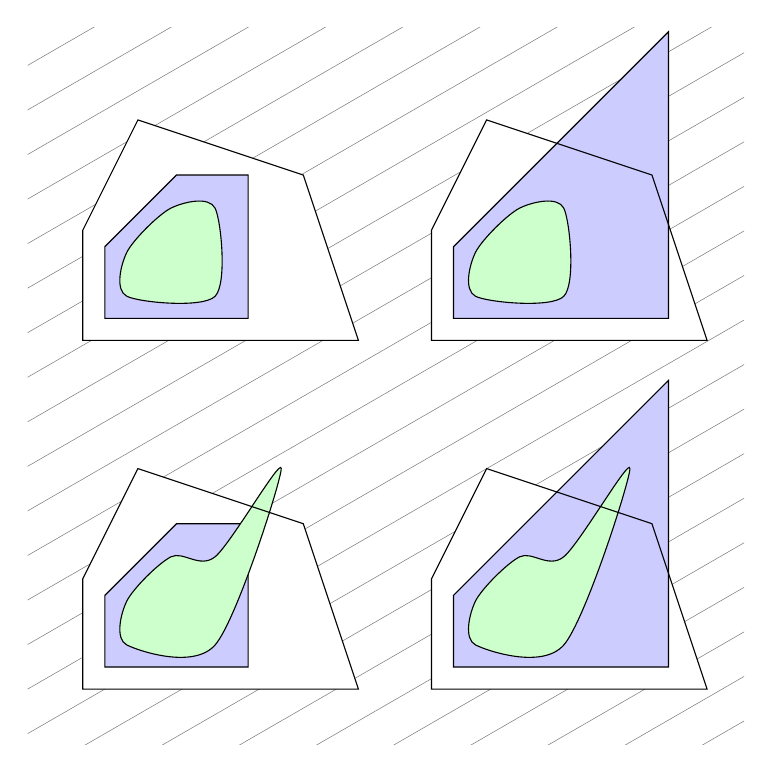
\begin{tikzpicture}[scale=0.7]
\clip  (-1,-1) rectangle (12,12);

% Hachures
\foreach \y in {-10,-9.3,...,11} \draw [gray, very thin, rotate=30] (-4,\y) to (18,\y);

% Ensemble sûr
\foreach \xsh in {0, 180}
\foreach \ysh in {0, 180}
\path [xshift=\xsh,yshift=\ysh,fill=white]
                 (0, 0) -- ++(0, 2)
            -- ++(1, 2) -- ++(3,-1)
            -- ++(1,-3) --    cycle;

% Approximation (précise)
\foreach \ysh in {0,180}
\draw [yshift=\ysh,fill=blue!20,scale around={1.3:(3,3)}]
                (1,1) -- (1,2)
             -- (2,3) -- (3,3)
             -- (3,1) -- cycle;

% Approximation (imprécise)
\foreach \ysh in {0,180}
\draw [xshift=180,yshift=\ysh,fill=blue!20,scale around={1.3:(3,3)}]
                (1,1) -- (1,2)
              -- (4,5)
             -- (4,1) -- cycle;

% Comportement réel (sans erreurs)
\foreach \xsh in {0, 180}
\draw [xshift=\xsh,yshift=180,fill=green!20,scale=0.8] plot[smooth cycle]
      coordinates{(1,1) (1,2) (2,3) (3,3) (3,1)};

% Comportement réel (avec erreurs)
\foreach \xsh in {0, 180}
\draw [xshift=\xsh,fill=green!20,scale=0.8] plot[smooth cycle]
      coordinates{(1,1) (1,2) (2,3) (3,3) (4.5,5) (3,1)};

% Ensemble sûr (redraw)
\foreach \xsh in {0, 180}
\foreach \ysh in {0, 180}
\draw [xshift=\xsh,yshift=\ysh]
                 (0, 0) -- ++(0, 2)
            -- ++(1, 2) -- ++(3,-1)
            -- ++(1,-3) --    cycle;

\end{tikzpicture}
\caption{Surapproximation. L'ensemble des états erronés est hachuré. L'ensemble
des états effectifs du programme, en vert, est surapproximé par l'ensemble en
bleu.}
\label{fig:staticanalysis}
\end{figure}

Le domaine ``sûr'' a une forme assez simple compte tenu des erreurs considérées:
c'est un produit d'ensembles simples, comme des intervalles. L'ensemble des
comportements réels du programme est au contraire d'une forme plus complexe
\footnote{D'ailleurs, en vertu du théorème de Rice, il n'est pas calculable.}.

En calculant une approximation de ce dernier, de forme plus simple, on peut
tester plus facilement que les comportements de sont dans la zone sûre : le fait
que l'analyse soit \emph{sound}, c'est à dire que l'approximation ne manque
aucun comportement, permet de prouver l'absence d'erreurs.

La figure~\ref{fig:staticanalysis} résume cette approche : l'ensemble des
valeurs dangereuses est représentée par un ensemble hachuré, l'ensemble des
comportements réels du programme est en vert, et l'approximation en bleu.

Plusieurs cas peuvent se produire. Ils correspondent aux cas suivants, de haut
en bas puis de gauche à droite :

\begin{itemize}
  \item on a prouvé, à la compilation, que le programme ne pourra pas comporter
  d'erreurs à l'exécution.
  \item l'analyseur doit émettre une (fausse) alarme. Il y a donc un manque de
  précision.
  \item l'approximation n'est pas \emph{sound}. Par construction, on évite ce
  cas.
  \item on signale un comportement erron\'e.
\end{itemize}

Toute la difficulté est donc de construire une surapproximation correcte mais
conservant une précision suffisante.

\jolibreak

% TODO check date Penjili

Le projet Penjili~\cite{AllamigeonHymansSSTIC07}, commencé à EADS Innovation
Works en 2005, a pour but de fournir un analyseur statique de logiciel système
embarqué critique utilisant l'interprétation abstraite pour prouver l'absence
d'erreurs à l'exécution.

Il a été employé pour vérifier la sûreté de plusieurs logiciels aéronautiques.

\jolibreak

Cependant, 

\subsection*{La solution retenue: \langname{}}

Dans le monde de l'aéronautique, il est nécessaire de s'assurer que les
logiciels embarqués critiques ne vont pas subir d'erreurs à l'exécution, dont
les conséquences financières et humaines peuvent être tragiques.

Afin de vérifier leur absence, des outils fondés sur l'interprétation abstraite
(section~\ref{sec:absint}) on été développés chez EADS Innovation Works dans le
cadre du projet Penjili~\link{penjili}. On y trouve notamment un langage
intermédiaire, Newspeak\cite{newspeak}, ainsi que des compilateurs permettant de
traduire du code C et Ada vers celui-ci. L'analyseur statique Penjili, reposant
sur ces outils, a été utilisé pour analyser des logiciels embarqués critiques de
plusieurs millions de lignes de code. Ce dernier n'est pour le moment pas open
source. Tous ces outils sont écrits dans le langage OCaml~\cite{DAOC}.

Les travaux présentés ici ont d'ailleurs été réalisés dans l'équipe de sécurité
et sûreté logicielle d'EADS Innovation Works, dans le cadre d'une convention
industrielle de formation par la recherche (CIFRE).

Nous avons choisi de baser notre analyse sur Newspeak, dans le but de bénéficier
de ces outils existants et dans la perspective de guider les analyses de valeur
par des information de typage.

Plus précisément, nous utilisons un langage nommé \langname, inspiré de Newspeak
mais avec un modèle mémoire de plus haut niveau permettant de garantir la sûreté
des programmes bien typés. L'implantation quant à elle se fait sur Newspeak.

\section{Plan de la thèse}

Cette thèse est organisée en trois parties. La première sert à décrire le
contexte de ces travaux, ainsi que les solutions existantes. La deuxième expose
notre solution, \langname, d'un point de vue théorique. La troisième rend compte
de la démarche expérimentale: comment la solution a été implantée et en quoi
elle est applicable en pratique.

\paragraph{Dans la partie~\ref{part:ctx},} on présente tout d'abord le
fonctionnement général d'un système d'exploitation. On y introduit aussi les
problèmes de manipulation de pointeurs contrôlés par l'utilisateur. Ceux-ci sont
centraux puisqu'on désire les restreindre. On fait ensuite un tour d'horizon des
techniques existantes permettant de traiter ce problème par analyse statique de
code source.

\paragraph{Dans la partie~\ref{part:lang},} on décrit notre solution:
\langname{}, un langage impératif. Sa syntaxe y est d'abord décrite, puis sa
sémantique ainsi qu'un système de types statiques. À ce niveau on a un bon
support pour décrire des analyses statiques sur un langage impératif. On étend
ensuite le système de types pour capturer les problèmes d'adressage mémoire
présents dans les systèmes d'exploitation. Pour ce faire, on ajoute des
pointeurs contrôlés par l'utilisateur à la sémantique et au système de types. À
chaque étape, c'est-à-dire avant et après ces ajouts, on établit une propriété
de sûreté de typage reliant la sémantique d'exécution aux types statiques.

\paragraph{Dans la partie~\ref{part:xp},} on documente la démarche expérimentale
associée à ces travaux. L'implantation du système de types sur le langage
\newspeak est d'abord décrite, à l'aide d'une variante de l'algorithme W de
Damas et Milner. La manière de compiler depuis du code C est également
présentée. Ensuite, on applique cette implantation à un cas d'étude concret. Il
s'agit d'un bug ayant touché un pilote de carte graphique dans le noyau Linux.
En manipulant incorrectement un pointeur dont la valeur est contrôlée par
l'utilisateur, il crée un problème de sécurité car un utilisateur malveillant
peut lire ou écrire dans l'espace mémoire réservé au noyau. En lançant notre
prototype, l'analyse de la version non corrigée lève une erreur alors que, dans
la version corrigée, un type correct est inféré. On montre ainsi que le système
de type capture précisément ce genre d'erreur de programmation.

On conclut enfin en décrivant les possibilités d'extension autant sur le point
théorique qu'expérimental.

% vim: spelllang=fr
